\section{Anwendungsschicht}
\begin{figure}[H]\centering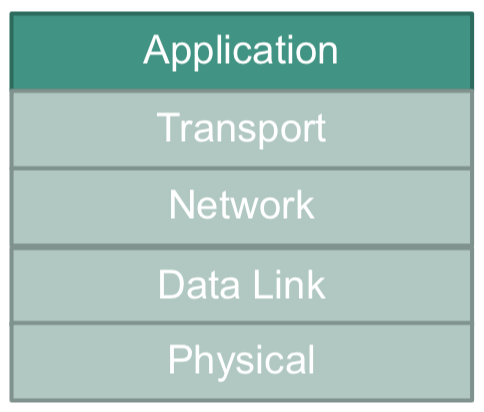
\includegraphics[width=80px]{SchichtAnwendung}\end{figure}

\paragraph{Historie}
\begin{items}
  \item \textbf{70er/80er}: Textbasierte Anwendungen (EMail, Remote Access)
  \item \textbf{90er}: World Wide Web, Instant Messaging, P2P-Filesharing
  \item \textbf{seit 2000}: steigende Vielfalt + Allgegenwärtigkeit: ($\Rightarrow$ Kritische Infrastruktur) \\* Voice over IP, Streaming, Gaming, Soziale Netzwerke, Smartphones
\end{items}

\paragraph{Schichtenmodell}
\begin{items}
  \item \textbf{Prozess}: Programm, das im Endsystem (Anwendungsschicht) abläuft
  \item \textbf{Nachricht}: Ausgetauscht zwischen Prozessen auf \emph{unterschiedlichen} Endsystemen
  \item Kommunikation in Schichten organisiert
  \item \textbf{Anwendungsschicht}: oberste Schicht \\*
    - enthält Anwendungsprotokolle \\*
    - Anwendung kümmert sich nicht um Datentransport
  \item \textbf{Datentransport}: unter Anwendungsschicht liegende Schichten \\*
    - Interna für Anwendung transparent \\*
    - Aber: Anwendung merkt Verzögerungen (Latenzen)
\end{items}

\paragraph{Verzögerung}
\begin{items}
  \item \textbf{Ausbreitungsverzögerung} \( t_a = \tfrac{d}{v} \) \\*
    \emph{Zeitspanne zwischen Absenden eines Signals und dessen Eintreffen am anderen \\* \phantom{-} Ende des Mediums} \\*
    Abhängig von: Ausbreitungsgeschwindigkeit \( v \), Länge des Mediums \( d \)
  \item \textbf{Sendezeit} \( t_s = \tfrac{X}{r} \) \\*
    \emph{Zeit zwischen Beginn und Abschluss der Sendung} \\*
    Abhängig von: Datenmenge \( X \), Datenrate des Mediums \( r \) \\*
    \textbf{Achtung}: Nach Sendungsabschluss sind die Daten noch nicht beim Empfänger! \\* \phantom{-} \( \leadsto \) Ausbreitungsverzögerung \( t_a \)
  \item \textbf{Verzögerung im Router} \\*
    - \emph{Pufferung} der Daten in Warteschlange \\*
    - \emph{Verarbeitung} (Fehlerüberprüfung usw.)
\end{items}

\paragraph{Protokollstack}
\begin{items}
  \item \textbf{Application}: SMTP, HTTP, XMPP,\dots
  \item \textbf{Transport}: TCP, UDP
  \item \textbf{Network}: IP
  \item \textbf{Data Link}: Ethernet, 802.11 (WiFi)
  \item \textbf{Physical}: Bits auf Medium
\end{items}

\paragraph{Socket und Interface}
\begin{items}
  \item \emph{Programmierschnittstelle für verteilte Anwendungen}
  \item Von OS bereitgestellte API
  \item Anwendungsprozess sendet/empfängt Nachrichten zum/vom Socket
  \item \textbf{Portnummern}: (De-) Multiplexing auf Endsystemen \\*
    Viele Prozesse auf einem Endsystem kommunizieren gleichzeitig über Netzwerk \\*
    \phantom{-} \( \leadsto \) eindeutige Socket-Identifikation über Portnummer
\end{items}

\paragraph{Client-Server-Anwendungen}
\begin{items}
  \item \textbf{Server}: Ständig in Betrieb, permanente IP-Adresse, häufig in Datenzentren
  \item \textbf{Clients}: Kommunizieren mit Server, \emph{nicht} direkt miteinander, dynamische IP-Adresse
\end{items}

\paragraph{Peer-to-Peer-Anwendungen}
\begin{items}
  \item Endysteme kommunizieren direkt miteinander \\*
    - Fordern Dienste von anderen Peers an und stellen selbst Dienste bereit \\*
    - Nicht permanent verbunden, wechseln dynamisch IP-Adressen \\*
    \phantom{-} \( \leadsto \) komplexes Management
  \item \textbf{Selbst-skalierend}: Neue Peers erhöhen Kapazität, fordern aber auch Dienste an
\end{items}

\paragraph{Web und HTTP --- Web-Dokumente}
\begin{items}
  \item Webseiten bestehen aus Basis-HTML-Datei und anderen Objekten (.js, .png,\dots)
  \item Jedes Objekt über URL (\emph{uniform resource locator}) referenzierbar
\end{items}

\paragraph{HTTP (Hypertext Transfer Protocol)}
\begin{items}
  \item ASCII-basiertes Transfeprotokoll der Anwendungsschicht im Web
  \item Basiert auf Client/Server-Modell \\*
    \emph{Client (Request)}: Browser, der Web-Objekte anfordert\\*
    \emph{Server (Response)}: Sendet über HTTP angeforderte Objekte
  \item Zustandslos: Jeder Request individuell, keine Zustandsinformation auf dem Server
  \item Kommunikation per TCP: \\*
    1. Client initiiert Verbindungsaufbau (Standard-Port: 80) \\*
    2. Server akzeptiert Verbindung \\*
    3. Austausch von HTTP-Nachrichten \\*
    4. Abbau der TCP-Verbindung
	\smallskip
  \item HTTP-Anfragen können verschiedene \textbf{Methoden} nutzen:
  \item \textbf{GET}: Ressource von Server zu Client übertragen (z.B. normale Webseite)
  \item \textbf{POST}: Daten zu Ressource übertragen (z.B. Web-Formular)
  \item PUT --- neue Ressource anlegen
  \item DELETE --- Ressource löschen
  \item HEAD --- wie GET, aber nur HTTP-Header übertragen
   \smallskip
  \item \textbf{Status-Codes:} Verarbeitungsindikator (Erfolg/Fehlschlag + Gründe)
  \item \textbf{200}: Erfolg; Antwort ist in dieser Nachricht
  \item \textbf{301}: Angefragtes Objekt wurde verschoben (neue URL in Nachricht spezifiziert)
  \item \textbf{400}: Server hat Anfrage nicht verstanden
  \item \textbf{404}: Angefordertes Objekt existiert nicht
  \item \textbf{505}: HTTP-Version nicht unterstützt
\end{items}
  \begin{figure}[H]\centering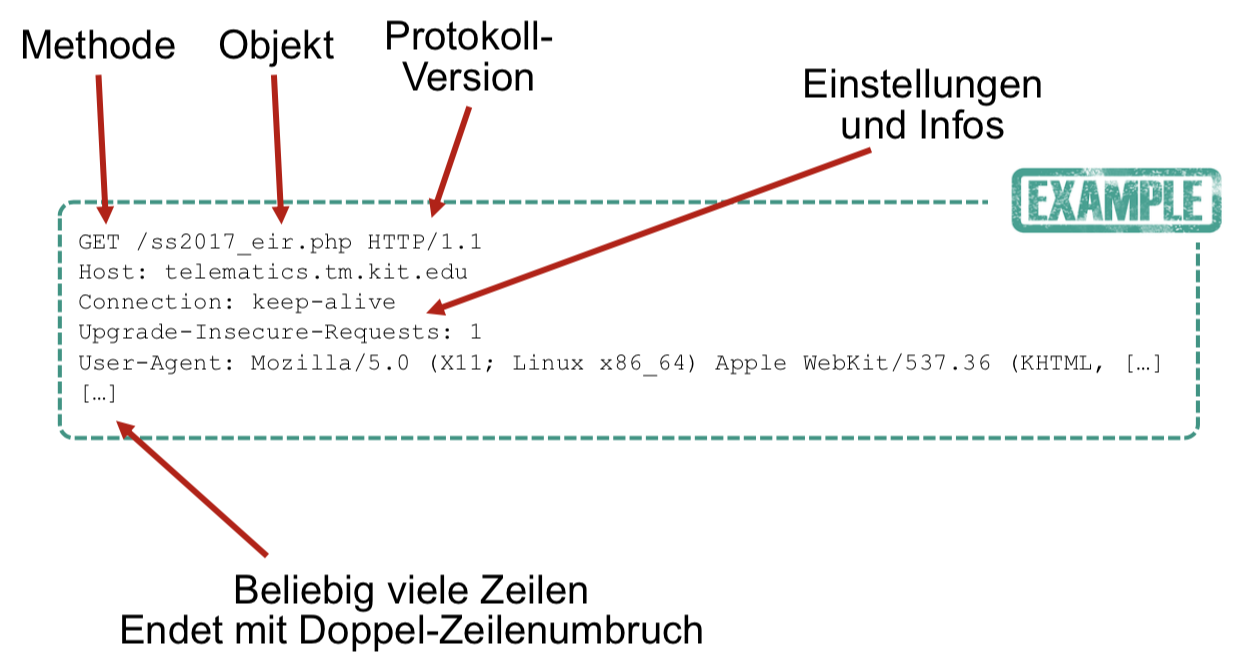
\includegraphics[width=0.33\textwidth]{HTTPRequest}\end{figure}
\begin{figure}[H]\centering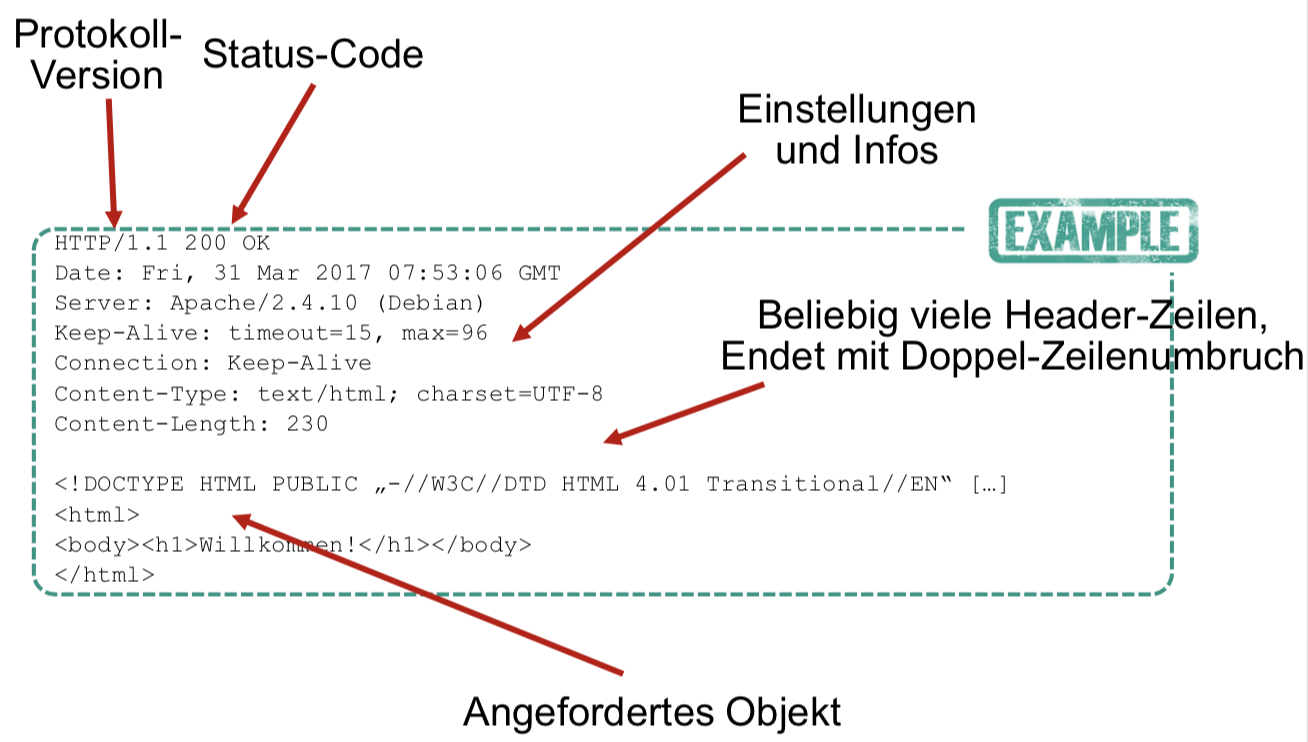
\includegraphics[width=0.33\textwidth]{HTTPResponse}\end{figure}

\paragraph{HTTP --- Verbindungen}
\begin{items}
  \item \textbf{Round Trip Time (RTT)}: Zeit, die Paket von Sender zu Empfänger und zurück benötigt
  \item \textbf{Non-persistent HTTP}: Höchstens ein Objekt über eine TCP-Verbindung, danach geschlossen \( \leadsto \) Mehrere Objekte erfodern mehrere TCP-Verbindungen (evtl. parallel)\\*
  \textbf{Antwortzeit}: \( 2*\text{RTT} + t_s \) pro Objekt\\*
  	- eine RTT für Verbindungsaufbau \\*
  	- eine RTT für HTTP-Anfrage und erste Antwortbytes \\*
  	- Zeit \( t_s \) für Senden des Objekts
  \item \textbf{Persistent HTTP}: Mehrere Objekte über eine TCP-Verbindung\\*
  \textbf{Antwortzeit}: Nur eine RTT für nachfolgende Objekte
\end{items}

\paragraph{HTTP --- Cookies}
\begin{items}
  \item \emph{Speichert Nutzer-Server-Zustand}
  \item \( \leadsto \) Server kann Inhalt abhängig von Nutzeridentifikation bereitstellen
  \item \textbf{Komponenten}: \\*
    - Cookie-Information in HTTP-Response-Nachricht (\textit{Set-Cookie}) \\*
    - Cookie-Information wird in nachfolgenden HTTP-Requests genutzt \\*
    - Datei mit Cookies wird auf Nutzer-Endsystem vom Browser verwaltet \\*
    - Datenbank bei Webseite \( \leadsto \) Server muss Cookies richtig interpretieren können
	\item \textbf{Privatsphäre: } Webseiten unterscheiden Nutzer durch Cookies \\*
    	\( \leadsto \) Werbeanbieter können Nutzer über viele Seiten tracken, viel über Nutzer lernen
\end{items}

\paragraph{Mail --- Komponenten}
\begin{items}
  \item \textbf{User Agent} (UA): Lesen, senden, weiterleiten
  \item \textbf{Mailserver}: User-Mailboxen, \emph{mail transfer agent} (MTA) / \emph{mail delivery agent} (MDA)
\end{items}

\paragraph{Mail --- SMTP (Simple Mail Transfer Protocol)}
\begin{items}
	\item Transfer von Mails zwischen Mailservern sowie vom User Agent zum Mailserver
  \item Drei Phasen: \\*
    1. Handshake \\*
    2. Nachrichtenübermittlung (E-Mail aus Header + Body) \\*
    3. Abschluss
  \item Client/Server-Model, Command/Response-Interaktionen \\*
    - Ähnlich Request/Response bei HTTP, nutzt ebenfalls TCP (Port 25) \\*
    - Kommandos: ASCII-Text \\*
    - Antwort: Statuscode + Nachricht
\end{items}
%\begin{figure}[H]\centering\label{SMTPAufbau}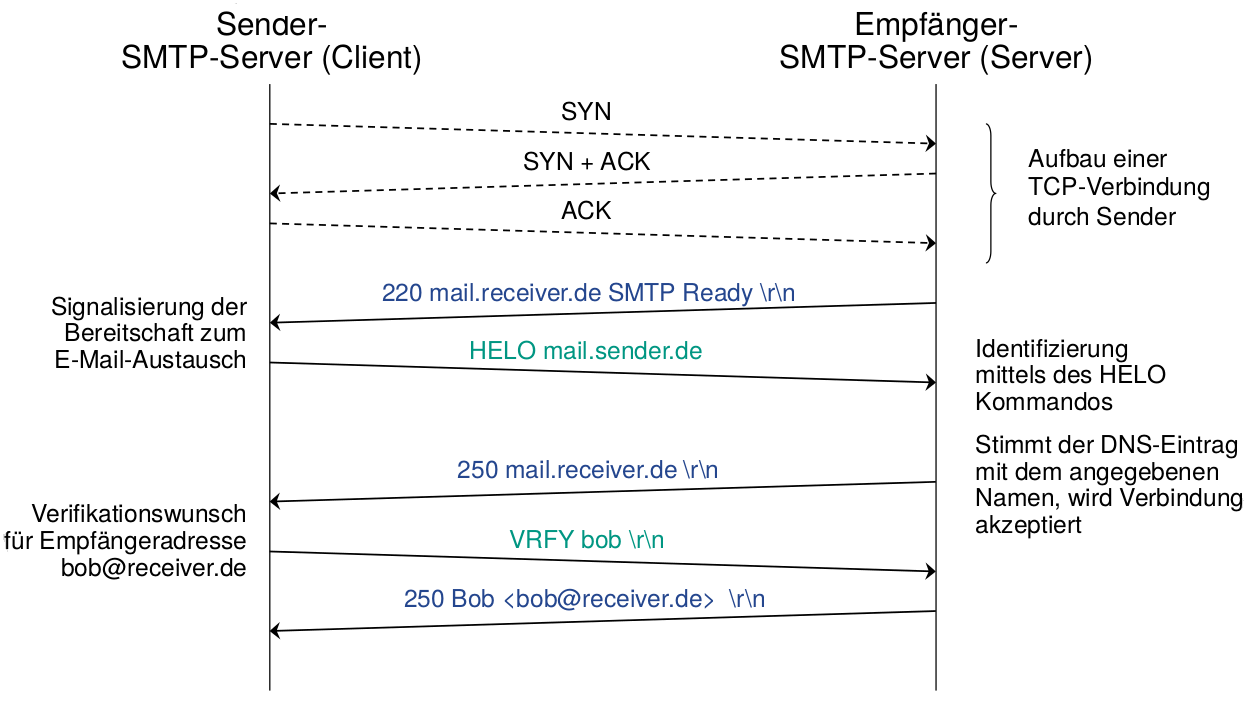
\includegraphics[width=0.33\textwidth]{SMTPAufbau}\end{figure}

\paragraph{Mail --- MIME (Multipurpose Internet Mail Exstensions)}
\begin{items}
  \item \textbf{Problem}: SMTP kann nur 7-Bit ASCII-Texte versenden, keine Dateien
  \item \textbf{MIME}: erweitert Kopfteil einer Nachricht um Formatinformation \\*
    \emph{Content-Type}: Definiert Typ des E-Mail-Inhalts; \emph{Content-Transfer-Encoding}
\end{items}

\paragraph{Mail --- Postfach-Abfrage}
\begin{items}
  \item \textbf{POP3} (\emph{post office protocol 3}): Verwaltung im UA, \emph{keine} Synchronisation\\*
    Client holt am Mailserver gespeicherte Nachrichten ab\\*
    nur einfache Funktionalität (\textit{list, retr, dele})
  \item \textbf{IMAP} (\emph{interactive mail access protocol}): Zentrale Verwaltung auf Mailserver\\*
    	Erweiterte Kommandos (Ordner, Filter)
   \item \textbf{Web-Mail}
\end{items}

\paragraph{WhatsApp --- XMPP (eXtensible Messaging and Presence Protocol)}
\begin{items}
  \item \emph{Echtzeit-XML-Streaming-Protokoll}
  \item Dezentral, ähnlich wie E-Mail
  \item Whatsapp nutzt einen Zentralen Server und proprietäre Variante des Protokolls
  \item \textbf{Clients}: zu ihrem jeweiligen Server verbunden
  \item \textbf{Server}: verbinden sich untereinander zur Nachrichtenübermittlung
  \item \textbf{Nachricht:} XML-Dokumente (erweiterbares Format)
  \item \textbf{Adressformat}: Server + Username, evtl. Client (z.B. alice@jabber.org/laptop)
\end{items}

\paragraph{DNS (Domain Name System)}
\begin{items}
  \item \textbf{Ziel}: Verwendung von Namen statt IP-Adressen
  \item \textbf{Aufgabe}: Zuordnung IP-Adresse \( \leftrightarrow \) Name (Subdomäne . Domäne . Top-Level-Domain)
  \item \textbf{Funktionalitäten}: \\*
    - \emph{Registrierung} von Namen + IP-Adressen \\*
    - \emph{Auflösung} von Namen in IP-Adressen\\*
    - \emph{Host Alias}: Löse einfacher zu merkende Alias-Namen in kanonische Namen auf\\*
    - \emph{Mail Server Alias}: Liefere E-Mail-Server zu einer Domain\\*
    - \emph{Lastverteilung}: Mehrere IPs von redundanten Servern in zufälliger Reihenfolge\\*
    \item Protokoll der Anwendungsschicht, über UDP (Port 53) realisiert, Client-Server-Modell
    \item Basisdienst, keine eigentliche Anwendung: Komplexität am Rand des Netzes
\end{items}

\paragraph{DNS --- Aufbau}
\begin{items}
	\item Probleme mit zentralem Server: Singuläre Fehlerquelle, Verkehrsaufkommen, geografische Entfernung, Verwaltungsaufwand, Abhängigkeit\\*
	
  \item Verteilte Datenbank in einer \textbf{Hierarchie} von Name-Servern (DNS-Servern)
  	\item \textbf{Lokaler Name-Server}: Erste Anfrage immer zu lokalem Server, Antwort aus eigener Zuordnungsdatenbank, dem Cache oder nach Befragung anderer DNS-Server
  	\item \textbf{Autoritativer Name-Server}: Enthält autoritative Abbildungen, jeder Host ist bei einem registriert (in seinem Netz)
  	\item \textbf{Top-Level Domain (TLD) Server}
  	\item \textbf{Root-Server}: Enthalten nur Einträge für TLDs, fixe IP-Adressen, 13 Root-Server-Cluster
\end{items}

\paragraph{DNS --- Anfragen}
\begin{items}
  \item \textbf{Rekursiv}: kennt angefragter Server Antwort nicht, fragt dieser weitere Server, bis er Antwort zurückliefern kann
  \item \textbf{Iterativ}: kennt ein Server die Antwort nicht, verweist er den \emph{Client} an andere Server
  \item \textbf{Üblich}: Client fragt lokalen Name-Server rekursiv, dieser dann iterativ
\end{items}

\paragraph{DNS --- Resource Records (RR)}
\begin{items}
  \item DNS ordnet Domänen zu Einträgen zu
  \item \textbf{A / AAAA} (Address): Abbildung Name auf IPv4/IPv6-Adresse
  \item \textbf{MX} (Mail Exchange): Mailserver einer Domäne (IP-Adresse)
  \item \textbf{NS} (Name Server): Nameserver einer Domäne (Hostname)
  \item \textbf{CNAME} (Canonical Name): Alias-Namen für Rechner/Domänen (Domain)
  \item \textbf{PTR} (Pointer): Abbildung IP-Adresse auf Name (Domain)
\end{items}

\paragraph{Content Delivery Networks (CDN)}
\begin{items}
	\item \textbf{Beispiel: Videostreaming} (hohe Datenrate, Datenqualität)
	\item \textbf{DASH (Dynamic, Adaptive Streaming over HTTP)}: Video aufgeteilt in Chunks, jeweils in mehreren Qualitäten (Bitraten) verfügbar, URLs und Infos in Manifest-Datei\\*
	Client wählt adaptiv bestmögliche Bitrate für jeden Chunk
	\item \textbf{Content Distribution}: Content zu hunderttausend Nutzern bringen
	\item Mega-Server: Skaliert nicht (Single Point of Failure, Netzwerküberlastung, Entfernung)
	\item \textbf{CDN:} Content auf geographisch verteilte Server kopieren\\*
		Third-Party CDNs (z.B. Akamei, Limelight), Private CDNs (z.B. Google für YouTube)
	\item Zwei Strategien:\\*
		- Enter Deep: Viele kleine Cluster in Zugangsnetzen nahe beim Nutzer\\*
		- Bring Home: Wenige große Cluster in wichtigen IXPs für geringeren Verteilungs- und Wartungsaufwand
	\item DNS-Manipulation: Autoritativer DNS-Server des CDN passt Antwort an IP-Adresse des anfragenden lokalen DNS-Server an, wählt einen nahe gelegenen CDN-Server aus
\end{items}